\chapter{Introduction}
\label{ch:introduction}

Wildlife@Home\footnote{http://volunteer.cs.und.edu/csg/wildlife/}~\cite{desell_2013_wildlife, desell_iccs_wildlife_2015} is a volunteer computing project in which citizen scientists and wildlife experts are presented videos taken from at the nests of various species of birds. Currently, users have the option of viewing Sharp-Tailed Grouse (\textit{Tympanuchus phasianellus}, an \textit{indicator species} which can represent ecological health), Interior Least Tern (\textit{Sternula antillarum}, a federally endangered species), or Piping Plover (\textit{Charadrius melodus}, a federally threatened species). Each of these species have different nesting behaviors and users are tasked with classifying them. Examples of behaviors are \emph{On Nest}, \emph{Off Nest}, \emph{Brooding}, \emph{Flying}, \emph{Foraging}, and \emph{Feeding}. While users are observing the nests, they create a time-series for each video specifying when these events begin and end. Each event in the time-series has a type, start time and end time (see Figure~\ref{fig:wildlife_interface}).

Such camera studies are popular in the field of avian ecology as they can reduce researcher impacts on animal behavior and also monitor animals in remote locations~\cite{cox-etal-2012, ellis-felege-carroll-2012}. Unfortunately, many of these studies are hampered by small sample sizes, where few have studied more than 100 nests~\cite{ellis-felege-carroll-2012}, limiting the biological inferences that can be made. In order to overcome these challenges, Wildlife@Home has been developed to employ both volunteer computing and crowd sourcing to quickly analyze wildlife video, as well as to investigate automated video analysis strategies using computer vision techniques.

\begin{figure*}
\centering
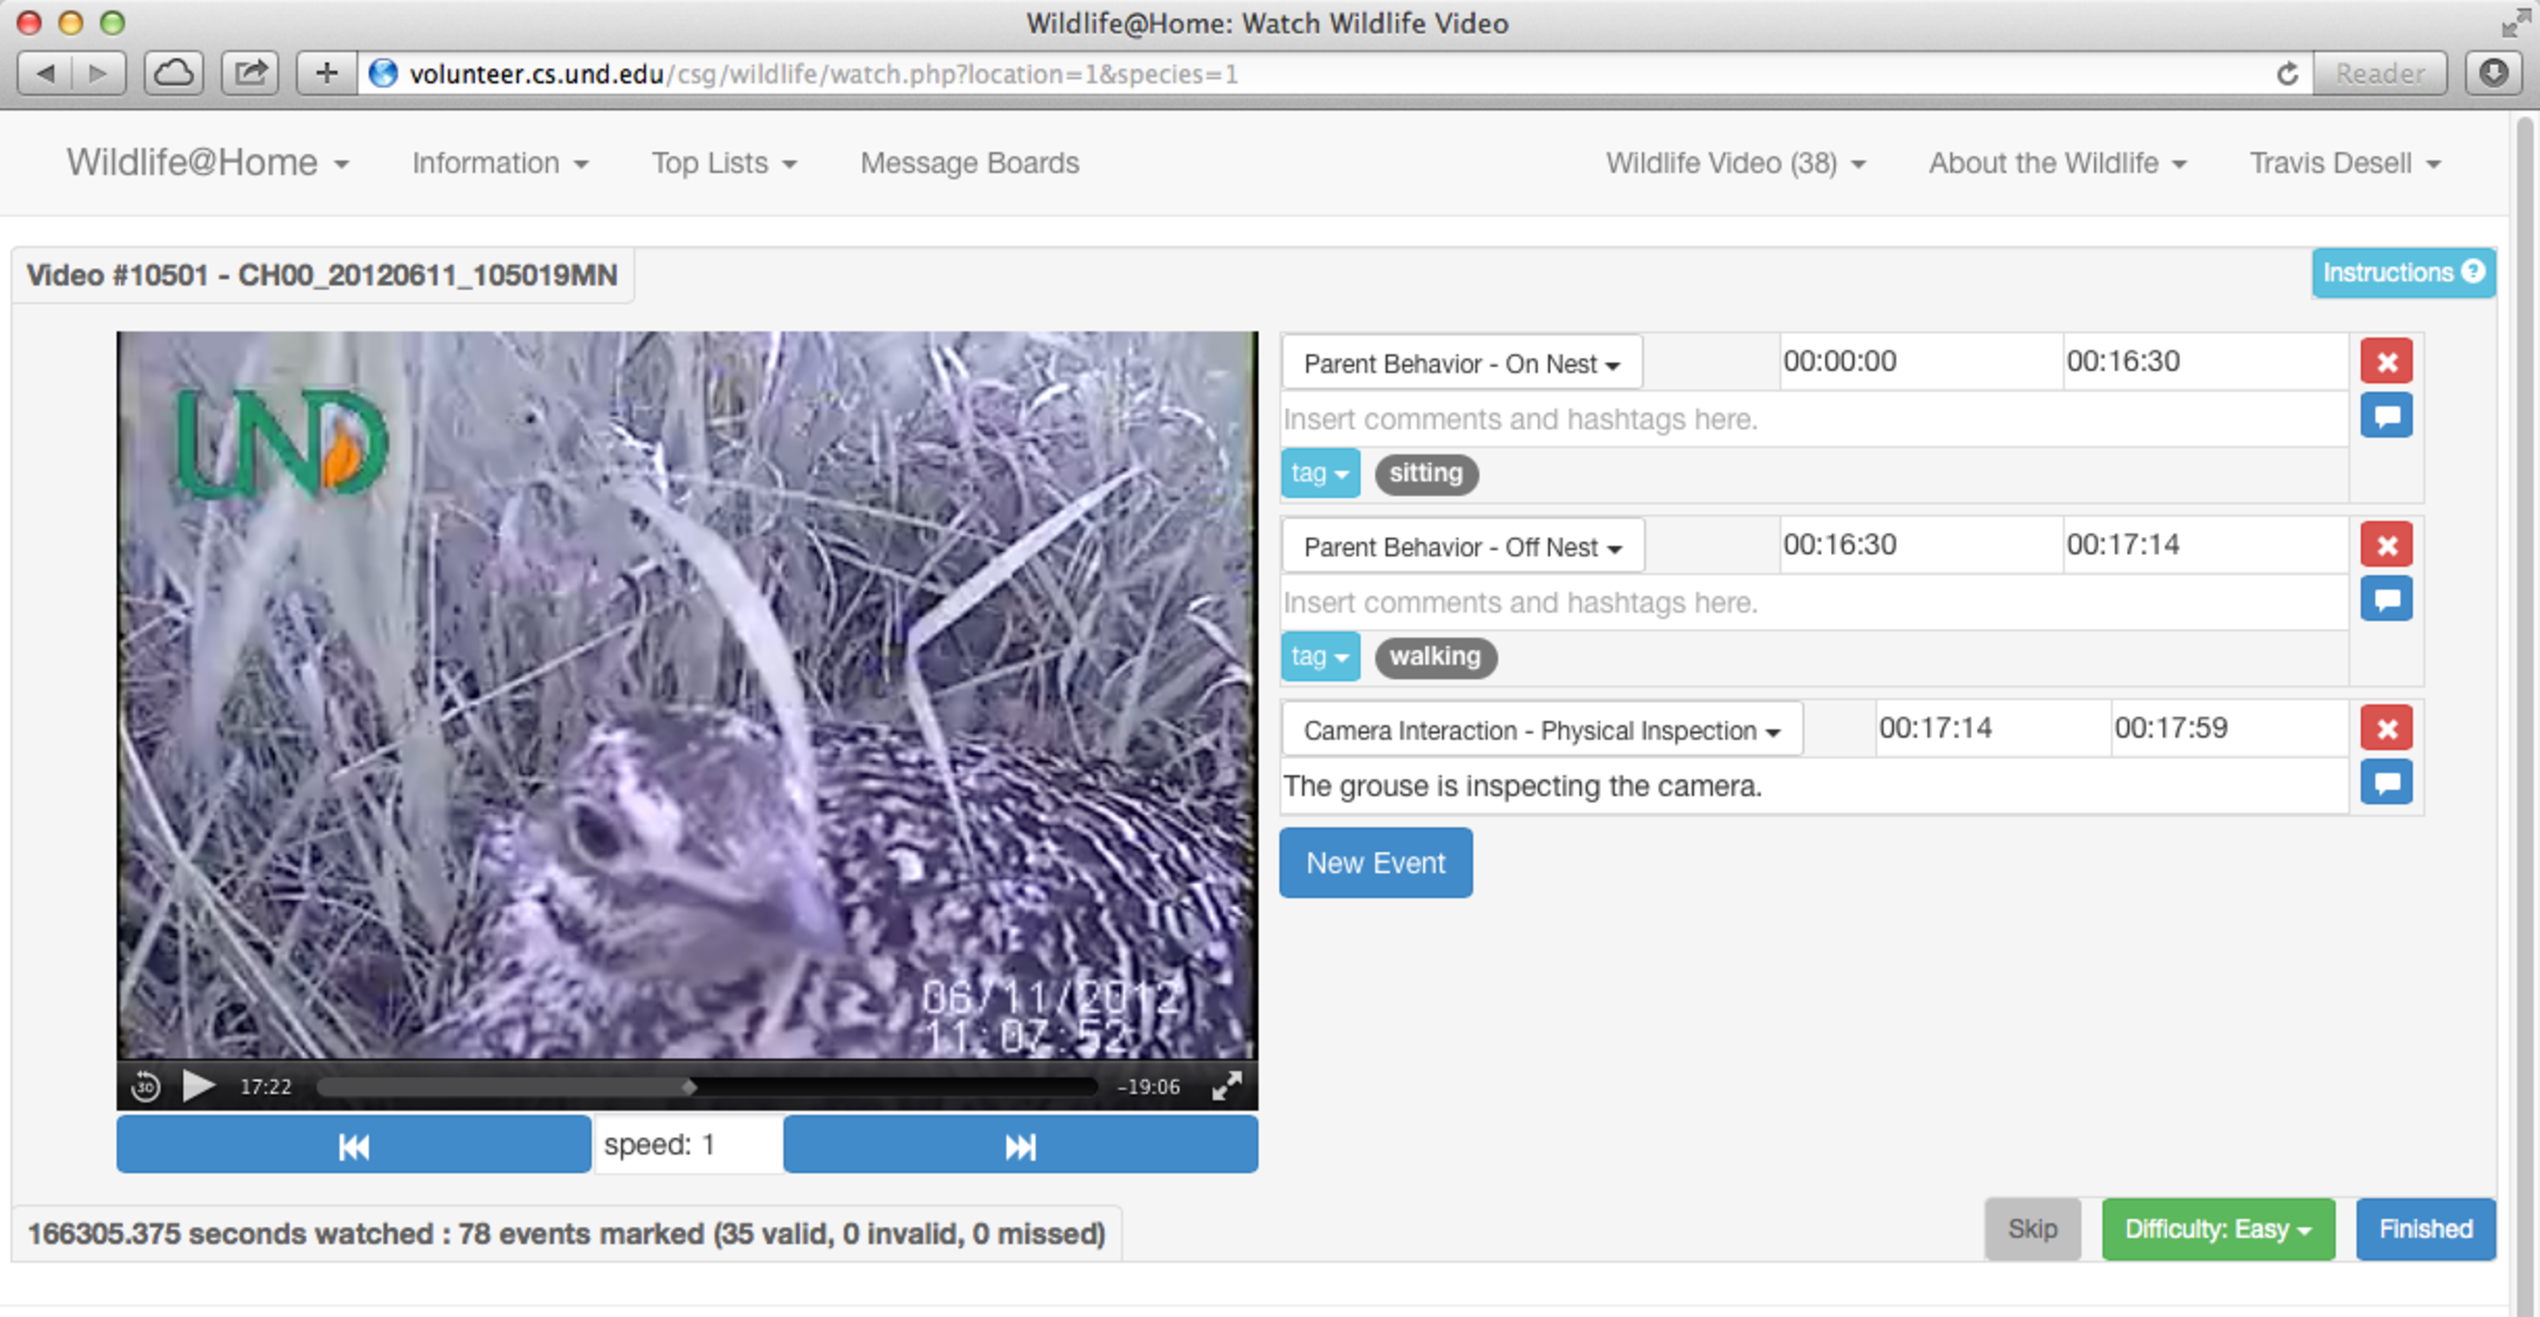
\includegraphics[width=5.8in]{./img/crowd_source_example_new.pdf}
\caption{An example of Wildlife@Home's video viewing interface. Users are shown 30 minute to 2 hour long nesting videos, and can specify the start and end time for various events of interest, and provide tags and comments for additional detail. Users can also specify how difficult it was to determine events for the video and discuss segments of the video on the project's message boards.}
\label{fig:wildlife_interface}
\end{figure*}

The Wildlife@Home project has accumulated over 85,000 hours of 24/7 uncontrolled outdoor surveillance video. This amount of data becomes problematic for humans to classify, even with software tools to help create and store event data. A lot of time is spent viewing regions of the video where the birds are not present at all or where a bird is present but highly inactive for long periods of time. Users watching video use the scrub bar to move more quickly through the video, especially uninteresting potions, and this can cause missed events. Scientists tasked with classifying long periods of uninteresting video can more quickly tire and lose focus.

This paper investigates the use of computer vision, machine learning, and background subtraction for the detection of avian nesting behaviors. The machine learning attempts to mimic the functionality of the human scientists by using image feature detection (SIFT~\cite{lowe_1999_object} \& SURF~\cite{bay_2006_surf}) and a support vector machine (SVM~\cite{burges_1998_tutorial, carpenter_2009_cusvm, chang_2007_psvm, chang_2011_libsvm}) to classify video frames. The background subtraction techniques focus on highlighting interesting or active section of video in order to aid scientists in behavior classification.

Feature detection and machine learning are effective for detection and classification of rigid objects~\cite{faro_2011_adaptive} but has also shown success in the recognition of pedestrians and some wildlife~\cite{heikkila_2004_real, dalal_2005_histograms, fan_2013_pedestrian,oren_1997_pedestrian, boom_2012_long}. We test the effectiveness of this method by using scientist observations as training data and compare algorithm performance in recognizing bird nesting behaviors.

Background subtraction is commonly used in surveillance video as a technique for segmenting objects of interest from a scene~\cite{mcivor_2000_background, piccardi_2004_background}. By extracting segments of the collected video with an abnormal amount of foreground activity, it is possible to algorithmically present scientists with video containing classifiable events and filter out video where no events occur.

While both methods focus on reducing scientist workload, they use very different methods to do so. The machine learning method attempts to determine an event type for each video frame by learning form previous classifications made by scientists. Each video frame is tagged with ongoing events and descriptors collected from that frame are used with a support vector machine to learn bird behaviors. The goal of this process is to automatically classify nesting behaviors, especially \emph{in video} and \emph{not in video} events. The background subtraction focuses on eliminating work for scientists by finding sections of video with bird activity or \emph{interesting} events. Background subtraction doesn't allow for classification of events but can greatly reduce scientist workload.

Feature detection with SURF and event classification with LIBSVM~\cite{chang_2011_libsvm} has shown to be a poor performer on the Wildlife@Home video. Many factors may cause poor performance on the footage, including video quality, brightness fluctuations, species cryptic coloration, and slightly incorrect event boundaries set by scientists. The poor results seen from this research sparked a shift to study the effectiveness of background subtraction in the same domain.

Given the diversity of species and nest locations, results find that background subtraction performance is sensitive to the amount of background movement, camera brightness, and cryptic coloration in a video. Using modern background subtraction techniques, such as Mixture of Gaussians (MOG)~\cite{power_2002_understanding}, and modified versions of the ViBe~\cite{van_2014_vibe} and Pixel-Based Adaptive Segmentation (PBAS)~\cite{hofmann_2012_background} algorithms, it is possible to show a strong correlation between scientist observed events and those calculated with background subtraction. By confidently narrowing the amount of video scientists are watching, it will be possible to focus on showing worth-while video segments and increase user incentive and focus.

Chapter~\ref{ch:related_work} presents modern techniques used for common feature detection algorithms, SVMs, and background subtraction problems. Chapter~\ref{ch:methodology} covers the approaches we took to classifying frames and extracting regions of the video with activity. Performance results and limitations of the algorithms are in described Chapter~\ref{ch:results}. Finally, Chapter~\ref{ch:conclusion} concludes with future work and a discussion of the next steps to collecting more results, improving the algorithms, and use of the data.

\begin{figure*}[!t]
\centering
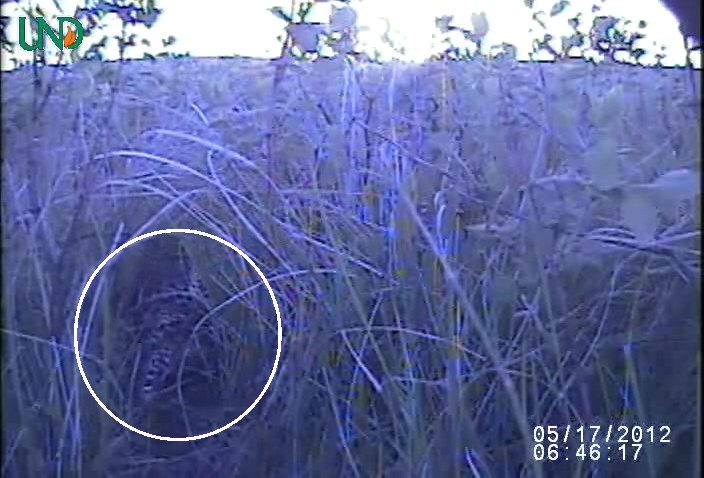
\includegraphics[width=2.5in]{6396_sample_grouse}
\caption{Sample Sharp-Tailed Grouse footage. The nest is marked with a white oval.}
\label{fig:sample_grouse}
\end{figure*}

\begin{sidewaysfigure}[!t]
\centering
\subfloat[Sample I]{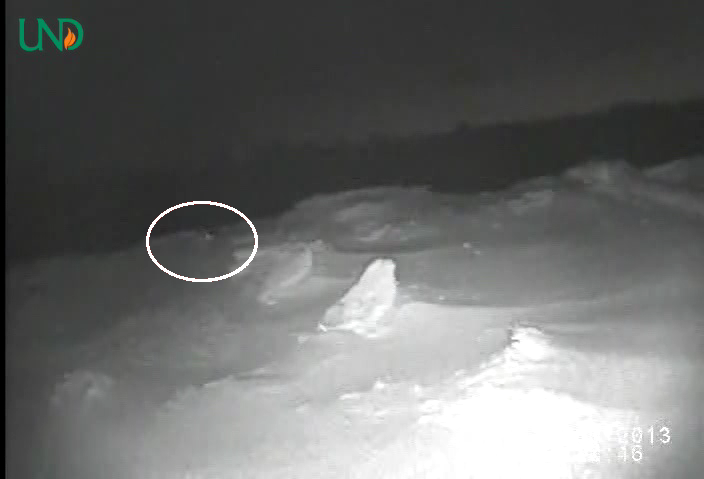
\includegraphics[width=2.9in]{59032_1}
\label{fig:first_case}}
\hfil
\subfloat[Sample II]{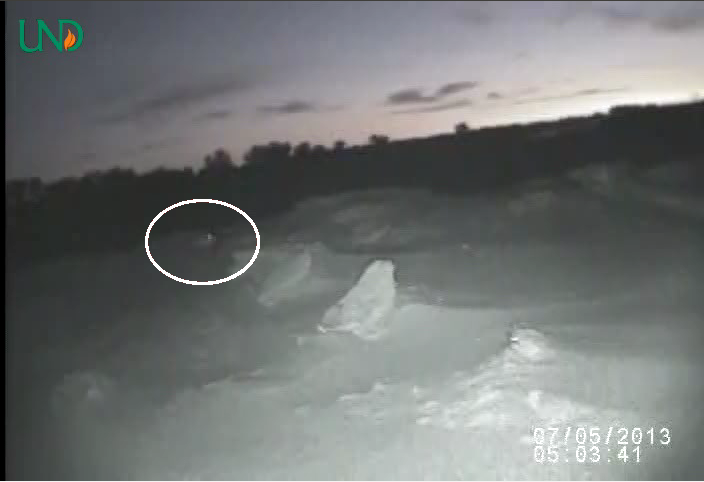
\includegraphics[width=2.9in]{59032_2}
\label{fig:second_case}}
\hfil
\subfloat[Sample III]{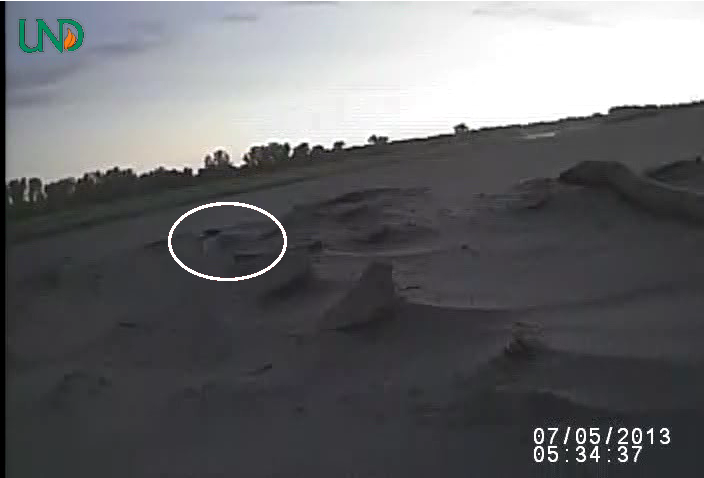
\includegraphics[width=2.9in]{59032_3}
\label{fig:third_case}}
\caption{Sample sunrise Interior Least Tern footage. The nest is marked with a white oval.}
\label{fig:example_tern_video}
\end{sidewaysfigure}

